\change{
	\section{Study Results}
	\stitle{RQ1: How \textit{informative} are the visualizations in the dashboard at providing users with an accurate understanding of unseen child visualizations?}
}
\npar \change{As discussed in Section~\ref{sec:problem}, an accurate and informative understanding of the ``root cause'' that led to the child distribution can help prevent users from falling prey to the drill-down fallacy. To this end,} the prediction task serves as a proxy for evaluating how accurately analysts understood the distributions present in various drill-down paths. In particular, we can get a sense of how \emph{informative} the dashboards were by examining how accurately participants could use visualizations present in the dashboard to predict an unseen visualization.
\par The accuracy of participants' predictions was measured by the Euclidean distance between the predicted distributions and ground truth data distributions. As shown in Figure~\ref{fig:distance} (left), predictions made using \system\ (highlighted in red) were closer to the actual distribution than compared to the baselines, as indicated by the smaller Euclidean distances. Figure~\ref{fig:distance} (right) also shows that \system participants \change{were able to more accurately reason about the expected properties of unseen data subsets, since they rated the resulting visualizations to be less surprising}. \cluster may have performed better in the Police dataset than it did in the Autism dataset due to the same reason as in the attribute ranking task, where more univariate visualizations happened to be selected.
\begin{figure}[h!]
\centering
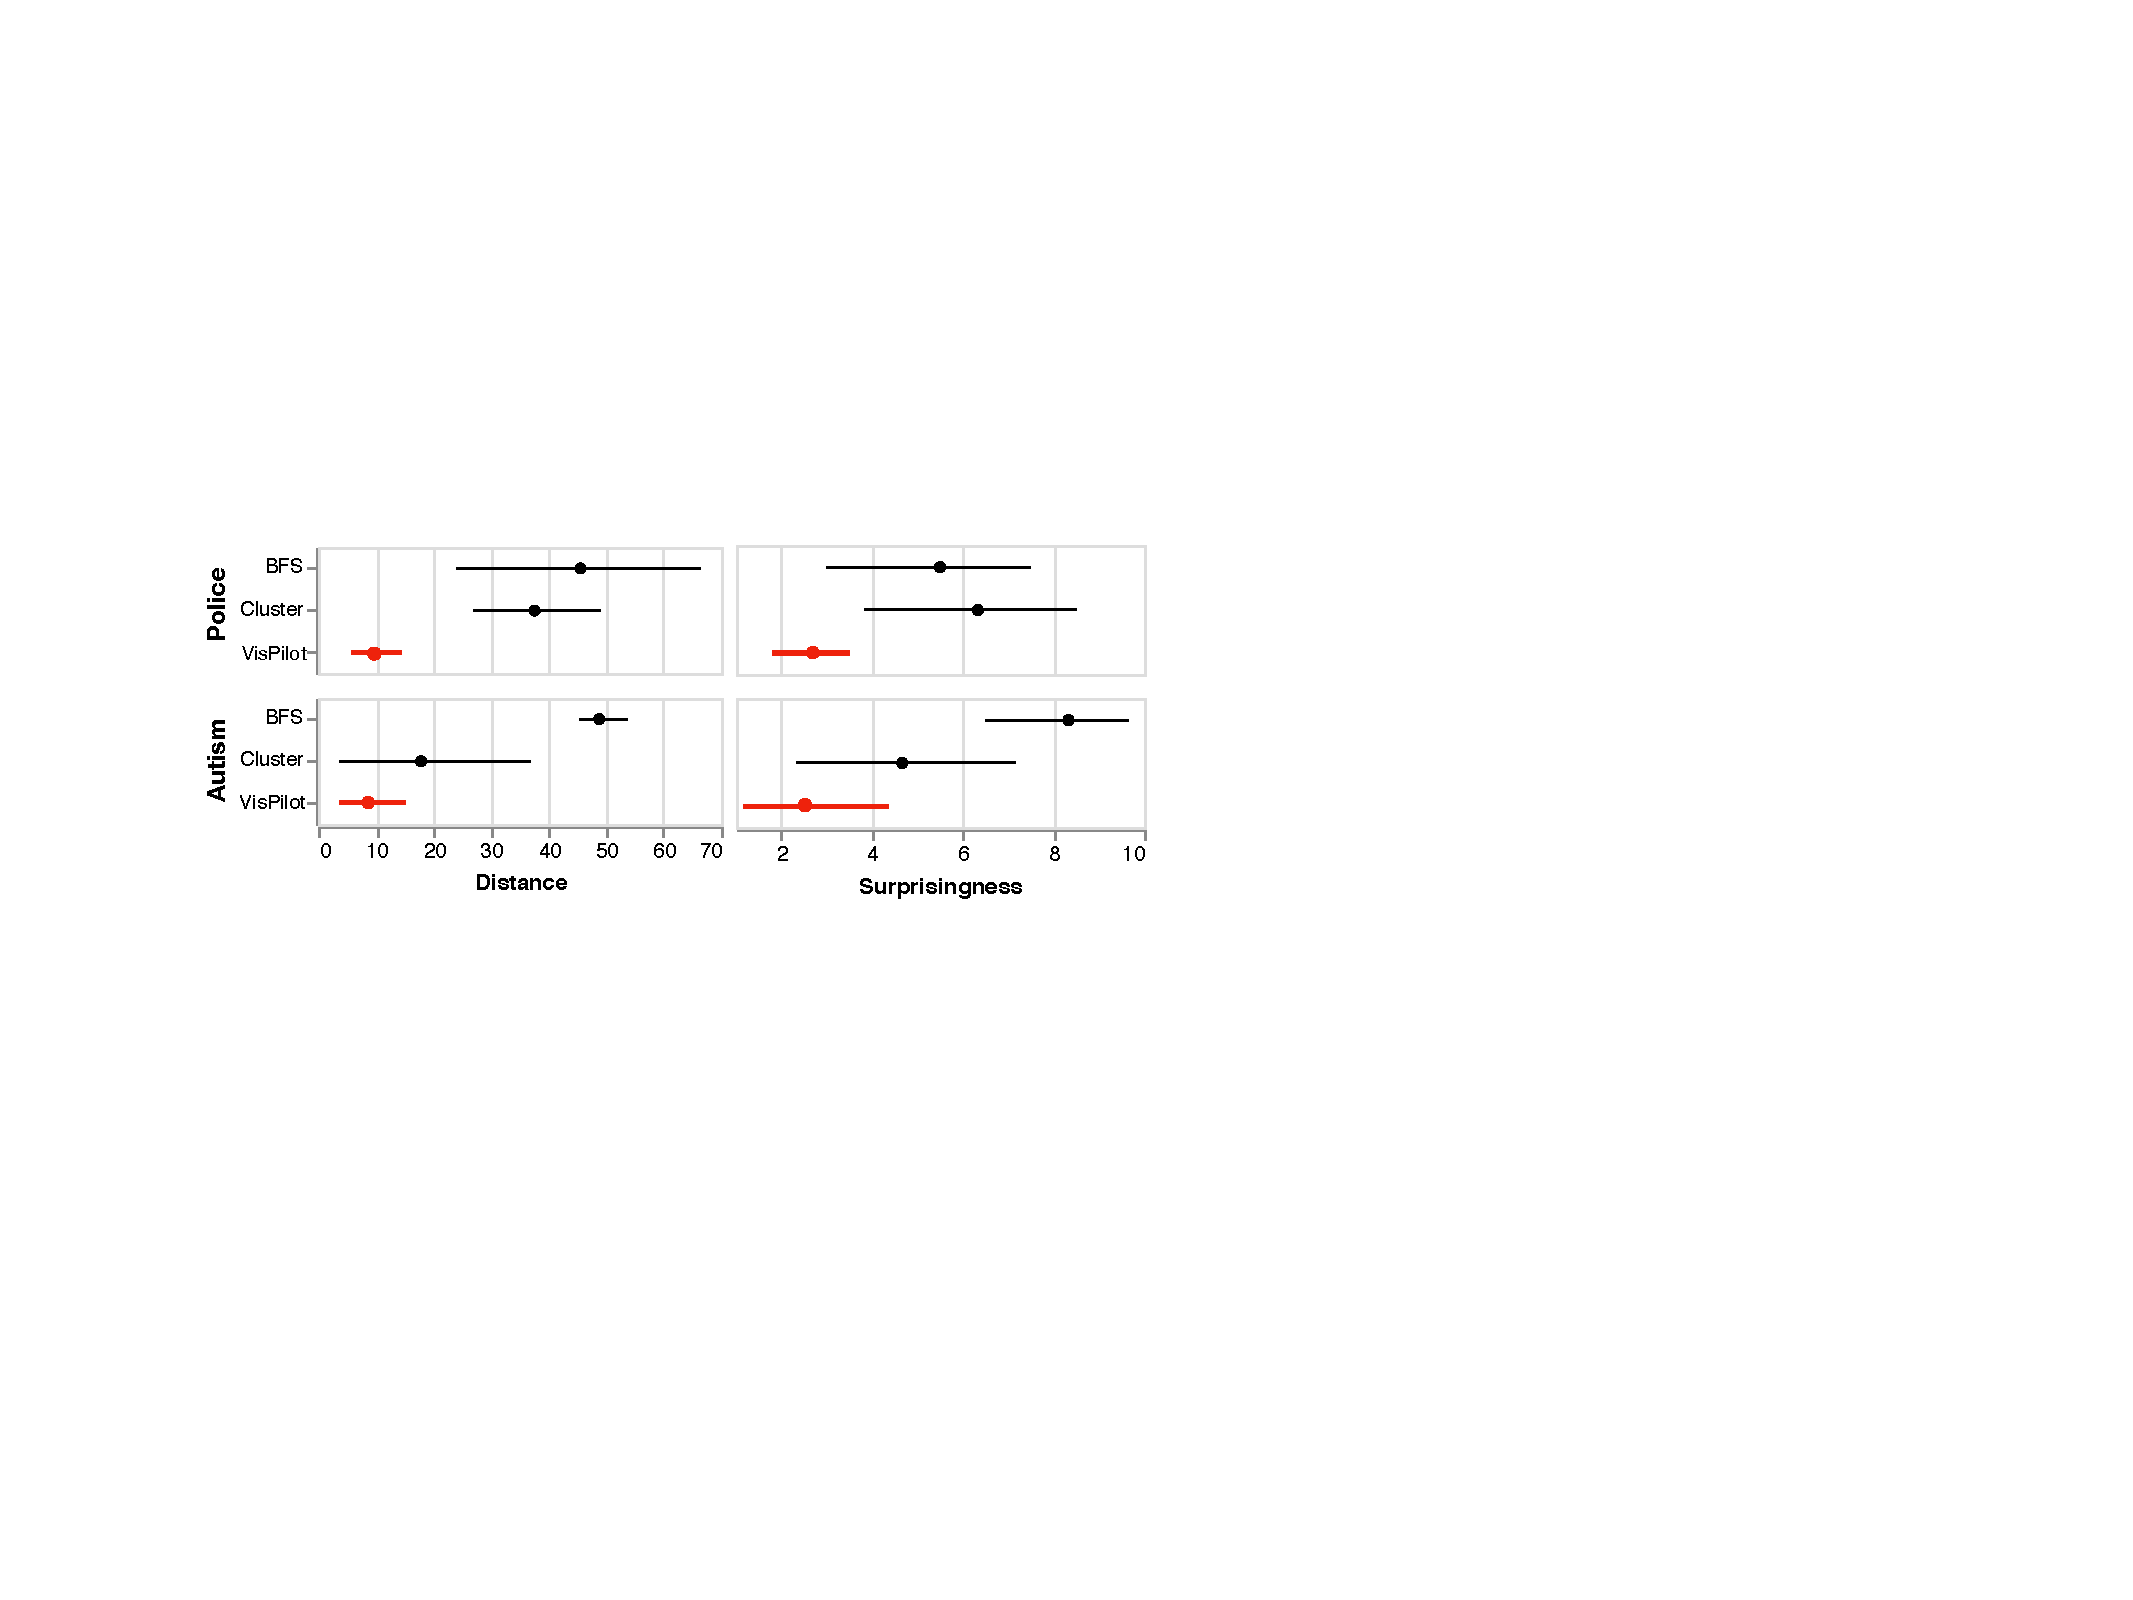
\includegraphics[width=0.95\linewidth]{figures/prediction_surprisingness_distance.pdf}
\caption{Left: Euclidean distance between predicted and ground truth. In general, predictions made using \system are closer to ground truth. Right: Surprisingness rating reported by users after seeing the actual visualizations on a Likert scale of 10. \system participants had a more accurate mental model of the unseen visualization and therefore reported less surprise than compared to the baseline.}
\label{fig:distance}
\end{figure}
\par We also compute the variance of participants' predictions across the same condition. In this case, low variance implies that any participant who reads the dashboard is able to provide consistent predictions, whereas high variance implies that the dashboard did not convey a clear data-driven story that could guide participants' predictions. So instead, participants \change{had to rely} on different priors or guessing to form their prediction. These trends can be observed in both Figure~\ref{fig:distance} and in more detail in Figure \ref{fig:actual_predictions}, where the prediction variance amongst participants who used \system\ is generally lower than the variance from the baselines.
\begin{figure}[h!]
\centering
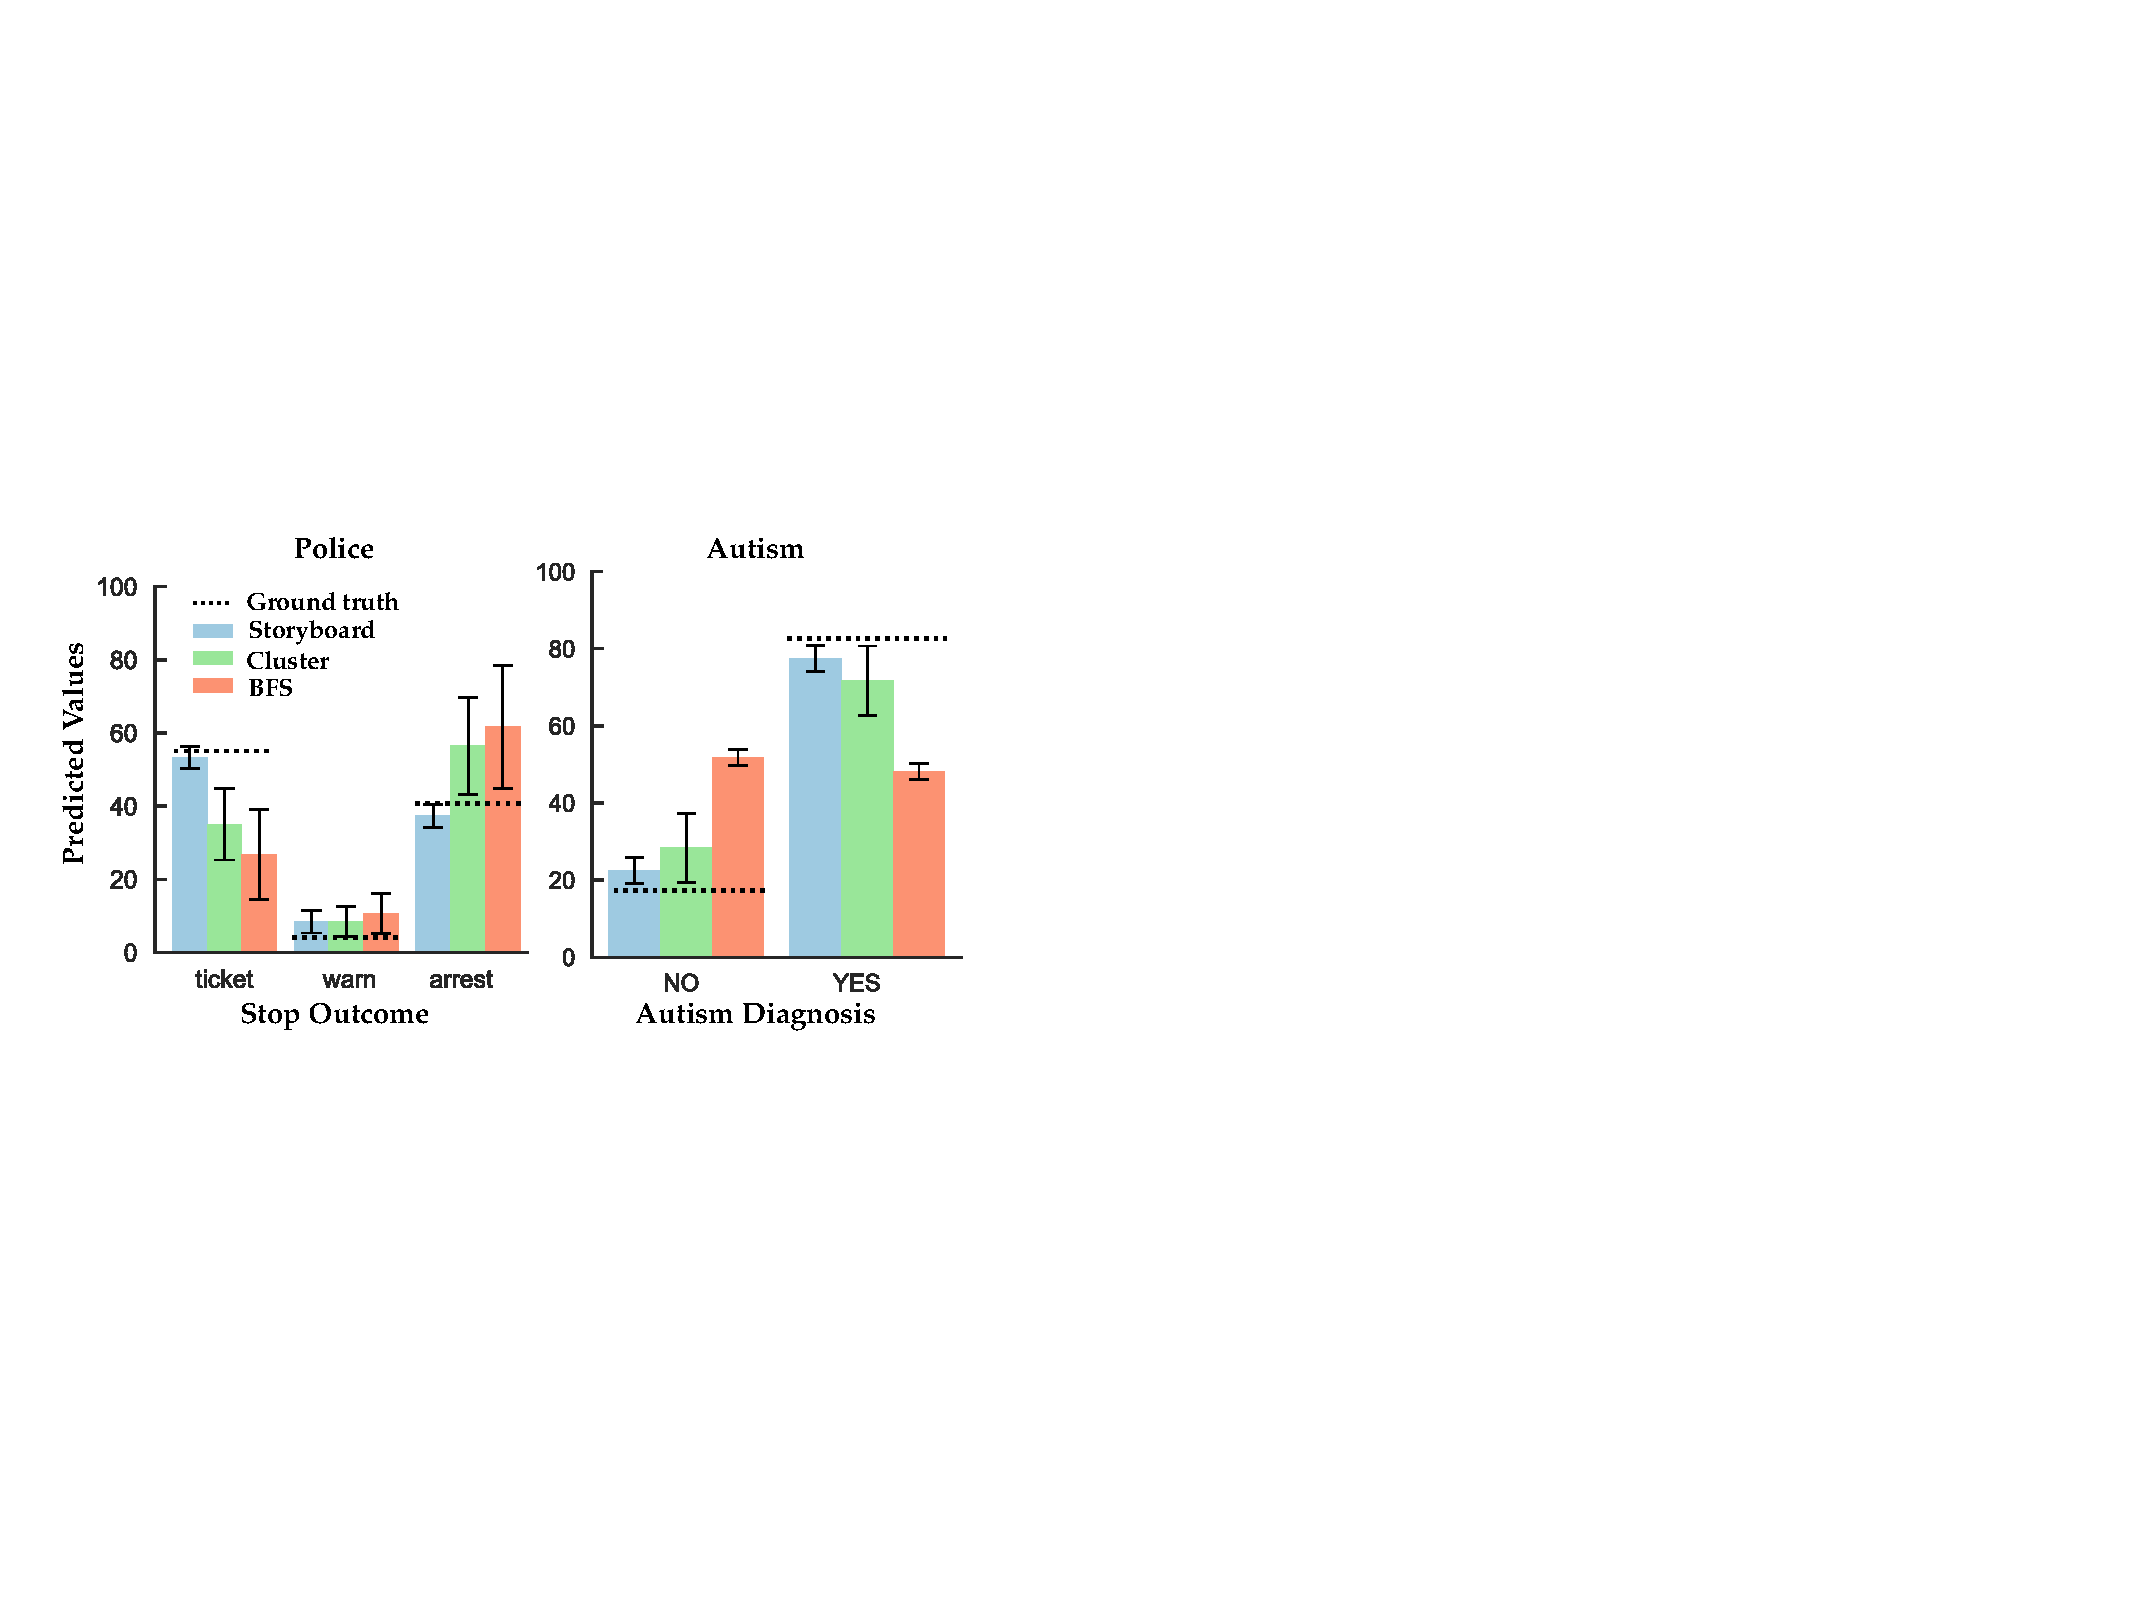
\includegraphics[width=0.85\linewidth]{figures/prediction.pdf}
\caption{Mean and variance of predicted values. Predictions based on \system exhibit lower variance \change{(error bars)} and closer proximity to the ground truth values (dotted).}
\label{fig:actual_predictions}
\end{figure}
\change{
	\stitle{RQ2: How well does the dashboard \textit{summarize} the relative importance of different attributes for a given dataset?}
	\npar For our study, we use the common analytical task of judging the relative importance of an attribute as an indicator of how well users are able to summarize key insights in a dataset based on the dashboard visualizations.
} To determine the attribute importance for a dataset, we computed the Cramer's V statistics between attributes to be ranked and the attributes of interest. Cramer's V is a common measure for determining the strength of association between categorical attributes~\cite{McHugh2013}. We deem an attribute as important if it has one of the top-three Cramer's V scores amongst all attributes of the dataset. This relevancy cutoff is visually-determined via the elbow method to indicate which rank the Cramer's V score drops off significantly. For the list of rankings provided by each participant, we first remove attributes where participants chose not to rank. Then we obtain the ground truth ranking based on the Cramer's V statistics for the ranked attributes. We compute the F-scores and average precision (AP) at k across a list of different k values (from 1 up to the number of ranked attributes, with k values corresponding to attributes ranked as ties deduplicated). Table \ref{table:ranking_results} summarizes the average across users in each condition, after picking the best performing k value for each user based on F-score and AP respectively. Both measures effectively capture how accurately participants were able to retrieve the three most important attributes for each dataset.
\begin{table}[ht!]
	\centering
	\begin{tabular}{|l|l|l|l|l|}
	\hline
	         & \multicolumn{2}{l|}{Police}                                   & \multicolumn{2}{l|}{Autism}                                   \\ \hline
	Metric   & F                             & AP                            & F                             & AP                            \\ \hline
	\system  & \cellcolor{blue!25}0.750 & \cellcolor{blue!25}0.867 & 0.723                         & 0.600                         \\ \hline
	\cluster & 0.739                         & 0.691                         & \cellcolor{blue!25}0.725 & \cellcolor{blue!25}0.665 \\ \hline
	\BFS     & 0.739                         & 0.592                         & 0.222                         & 0.200                         \\ \hline
	\end{tabular}
	\caption{Best AP and F-scores for the attribute ranking task.}
	\vspace{-10pt}
    \label{table:ranking_results}
\end{table}
\par Even though \BFS has inherent advantage for this task since \BFS dashboards consist of all univariate distributions, which provides more high-level information regarding each attribute, both \system and \cluster (which contained more `local' information) performed better than \BFS for both datasets. The problem with \BFS is that given the limited number of visualizations that could be shown on a dashboard, not all univariate distributions can be exhaustively shown. For the Police dataset, it happened to select several of the important attributes (related to contraband and search) to display in the first 10 visualizations. However, with a budget of k=10, only visualizations regarding binary diagnostic questions 1-4 fit in the dashboard for the Autism dataset. So the poor ranking behavior comes from the fact that the \BFS generated dashboard failed to display the three most important attributes (questions 5, 6 and 9) given the limited budget. This demonstrates \BFS's lack of providing a guarantee especially when exhaustive exploration has a limit (e.g., time or attention of analyst).
\par We see that \system\ performs better than \cluster for the Police dataset and closely follows \cluster for the Autism dataset. It is not entirely surprising that \cluster did well, since it is a well-established method for summarizing high-dimensional data~\cite{Han2005}. For the Autism dataset, \cluster happened to pick the majority of visualizations (8/10) as univariate distributions that exhibited high-skew and diversity, leading to more informed inference on attribute importance. Since clustering seeks visualizations that exhibit diversity in the shape of the data distributions, it could potentially result in visualizations with many filter combinations. For the police dataset, 6 out of 10 visualizations had 2-4 filters, making it difficult for analysts to interpret without appropriate context to compare against.
\par Both \BFS and \cluster do not provide consistent guarantees for highlighting important visualizations across different datasets. In general, our results indicate that users gain a better understanding of attribute importance using \system, with only a few targeted visualizations that tells the `whole story'. Note that this is without \system being explicitly optimized for this ranking purpose.

\change{\stitle{RQ3: How \emph{interesting} are the visualizations in the dashboard perceived subjectively by the users?}
}
\npar Using the click-stream data logged from the user study, we recorded whether a
participant \change{labelled} a visualization in the dashboard as interesting, not interesting, or left the visualization unselected. Table~\ref{table:interestingScore} summarizes counts of visualizations marked as interesting or not interesting aggregated across conditions. We also normalize the interestingness count by the total number of selected visualizations to account for variations in how some participants select more visualizations than others. The results indicate that participants who used \system\ had more visualizations that they found interesting compared to the \BFS and \cluster condition. \change{While the labelling task is inherently subjective and there are numerous reasons why a participant may have marked a visualization as interesting or uninteresting, this result is an indication } that \system's \textit{saliency} objective was able to select visualizations that were perceived as interesting to the users.
\begin{table}[h!]
	\centering
	\begin{tabular}{|l|rrr|}
	\hline
	 \small{Condition}             &   \small{\system} &   \small{\BFS} &   \small{\cluster} \\
	\hline
	 \small{Interesting}            &  \cellcolor{blue!25}       66    & 61    &      51   \\
	 \small{Not Interesting}        &  \cellcolor{blue!25}       10    & 20    &      22   \\
	 \small{Interesting (Normalized)} &   \cellcolor{blue!25}       0.87 &  0.75 &       0.7 \\
	\hline
	\end{tabular}
	\caption{Total counts of visualizations marked as interesting or not interesting across the different conditions. \system leads to more visualizations marked as interesting and fewer visualizations marked as uninteresting.}
	\label{table:interestingScore}
\end{table}
